\documentclass[11pt,a4paper]{article}

% --- packages ---------------------------------------------------------
\usepackage[utf8]{inputenc}
\usepackage[T1]{fontenc}
\usepackage[margin=1in]{geometry}
\usepackage{amsmath,amssymb,amsthm}
\usepackage{bm}
\usepackage{mathtools}
\usepackage{booktabs}
\usepackage{array}
\usepackage{xcolor}
\usepackage{graphicx}
\usepackage{float}
\usepackage{caption}
\usepackage{subcaption}
\usepackage{enumitem}
\usepackage{microtype}
\usepackage{hyperref}
\hypersetup{colorlinks=true,
            linkcolor=blue!50!black,
            citecolor=blue!50!black,
            urlcolor=blue!50!black,
            pdftitle={Cascaded chi3 SH-only metasurface -- sample analysis}}

% --- macros (kept identical to the simulation report) -----------------
\newcommand{\eps}{\varepsilon}
\newcommand{\bvec}[1]{\mathbf{#1}}
\newcommand{\f}{\bvec{f}}
\newcommand{\chitwo}{\chi^{(2)}}
\newcommand{\chithree}{\chi^{(3)}}
\newcommand{\Dom}{\Delta\omega}
\newcommand{\geom}{{\rm geom}}
\newcommand{\chicasc}{\chithree_{\text{casc}}}
\newcommand{\etag}{\eta_{\geom}^{(1\mathrm R)}}
\newcommand{\Eloc}{E_{\text{loc}}}

% Caption styling
\captionsetup{labelfont={small,bf}, font=small, labelsep=period}

% Spacing
\setlength{\parskip}{0.4em}
\setlength{\parindent}{0pt}
\emergencystretch=3em   % absorb sub-em paragraph overfulls

% Paragraph headers a touch lighter
\makeatletter
\renewcommand\paragraph{%
  \@startsection{paragraph}{4}{\z@}%
                {1.0ex \@plus 0.5ex \@minus .2ex}%
                {-0.6em}%
                {\normalfont\itshape}}
\makeatother

% Path to simulation figures (PDF)
\graphicspath{{../cascaded_chi3/figures/samples/}{../cascaded_chi3/figures/}}

% =====================================================================
\begin{document}

\title{Cascaded $\chitwo{:}\chitwo \to \chithree_\text{eff}$ in Singly-Resonant
       LiNbO$_3$ Metasurfaces\\[2pt]
       \large Sample Analysis (fabricated designs 1--4)}
\author{}
\date{\today}
\maketitle

\begin{abstract}
\noindent
A numerical companion to \texttt{Cascaded\_chi3\_SH\_only\_note.tex}, applying the
singly-resonant (SH-only) cascaded-$\chithree$ model to four fabricated LiNbO$_3$
metasurface designs supplied by the designer (samples~1--4, pump
$\lambda_1\!\approx\!0.97$--$1.06\,\mu$m). Parameters are extracted from the
COMSOL transmission spectra, the nonlinear overlap integrals, and the LiNbO$_3$
dispersion table; the full extraction and consistency checks are documented in
\texttt{SH\_only\_sample\_parameters.md}. We evaluate every observable that
\emph{survives} the loss of the fundamental resonance --- the effective
$\chicasc(\Dom)$ and its sign-flip, the two-photon-like loss, the
bandwidth-integrated strength, the single-pass Kerr phase, saturable absorption,
FWM, and SHG conversion --- and locate the optimal operating detuning per sample.
The headline is that the cascade is a \emph{material enhancement of a few to
ten} ($R^{(1\mathrm R)}\!=\!|\chicasc|/\chithree_{\rm native}\!\approx\!1.5$--$10$,
limited by an overlap $2$--$10\times$ below the value assumed in the note;
these values include the October 2026 factor-$4$ correction of the cascaded
prefactor, \S\ref{sec:spectra}), that no single-pass
Kerr \emph{device} is observable, and that the highest-leverage design change is
to raise the nonlinear overlap. All formulae are cross-checked against the
note and an independent re-derivation (\S\ref{sec:verify}). Absolute magnitudes
carry an $\mathcal{O}(1)$ normalisation-bridge uncertainty pending one absolute
SHG-efficiency datum (\S\ref{sec:open}).
\end{abstract}

\tableofcontents
\bigskip

% =====================================================================
\section{Samples and parameter extraction}
\label{sec:samples}

The four samples share a 400\,nm lattice period and a LiNbO$_3$ meta-atom (base
$H_1$ + pillars $H_2$, total thickness $H_t$) on which only the second harmonic is
resonant; the fundamental sits in the linear transmission band (measured FM
transmission $|t|^2\!\approx\!0.73$, flat to $<\!1.3\%$, confirming the SH-only
premise). The active tensor component is $\chitwo_{zzz}=2d_{33}$ along the
extraordinary axis ($E_z$ out-of-plane), so $n_1=n_e(\lambda_1)$,
$n_2=n_e(\lambda_2)$ from the supplied Sellmeier table. Frequencies satisfy
$\omega_1=\pi f_0(2\omega)$, $\gamma_2 = \omega_2/Q_2 = 2\pi\gamma[\text{THz}]$,
and the usable Kerr bandwidth $\Delta f = \gamma_2/2\pi = \gamma[\text{THz}]$.

\begin{table}[H]
  \centering
  \caption{Per-sample model parameters (files \texttt{design4\_<geometry>.mat}).
  $\etag$ from the COMSOL overlap at $\Dom=+2\gamma_2$ (baseline normalisation
  $C_{\rm bridge}=1$); material baseline $|\chitwo|=5\times10^{-11}\,$m/V,
  $\chithree_{\rm native}=2\times10^{-21}\,$m$^2$/V$^2$.}
  \label{tab:params}
  \small
  \setlength{\tabcolsep}{5pt}
  \begin{tabular}{llcccccc}
    \toprule
    S & geometry & $\lambda_1$ & $\lambda_2$ & $Q_2$ &
      $\Delta f$ & $L_{\rm meta}=H_t$ & $\etag$ \\
    \midrule
    1 & \texttt{alpha9}          & 997\,nm  & 498\,nm & 3442 & 175\,GHz & 190\,nm & 0.0144 \\
    2 & \texttt{H1\_70}          & 975\,nm  & 488\,nm & 3486 & 176\,GHz & 180\,nm & 0.0112 \\
    3 & \texttt{H1\_120\_H2\_100} & 1058\,nm & 529\,nm & 4641 & 122\,GHz & 220\,nm & 0.0375 \\
    4 & \texttt{H1\_140\_H2\_80}  & 1064\,nm & 532\,nm & 5633 & 100\,GHz & 220\,nm & 0.0437 \\
    \bottomrule
  \end{tabular}
\end{table}

\paragraph{Overlap mapping.}
The designer's normalised overlap,
\begin{equation*}
  \text{overlap}=\frac{1}{A}\,
    \frac{\iint E_z(\omega)\,E_z(\omega)\,E_z^{*}(2\omega)\,dA}
         {|E_z(\omega)|\,|E_z(\omega)|\,|E_z(2\omega)|}\,,
\end{equation*}
is exactly the SH-only SHG overlap $\widetilde M$ of the note
(Eq.~\texttt{Mtilde-def}), normalised. Since $\chicasc\propto|\widetilde M|^2$, the
geometric overlap is $\etag(\Dom)=(|\text{overlap}|/A)^2\,C_{\rm bridge}$,
evaluated at the SH frequency $f=f_0+\Dom/2\pi$. The resonant amplitude is
divided out in the designer's definition, so the overlap is the \emph{spatial
coherence factor only}; the resonant build-up is supplied by the model's
$1/(\Dom+i\gamma_2/2)$. Reproducing $|\text{overlap}|/A$ at $f_0\pm2\gamma$ from
the raw arrays matches the designer's table to within $\pm6\%$ (one tabulated
value, sample~2 at $-2\gamma$, is a decimal typo: $0.9000\to0.0900$).

% =====================================================================
\section{Cascaded \texorpdfstring{$\chithree$}{chi3} spectra}
\label{sec:spectra}

With $\etag(\Dom)$ from the overlap data, the effective susceptibility is
\begin{equation}
  \chicasc(\Dom)\;=\;-\,\frac{2\,\omega_1|\chitwo|^2\,\etag(\Dom)}
                              {3\,n_2^2\,(\Dom+i\gamma_2/2)}\,,
  \label{eq:chi3}
\end{equation}
(prefactor $2/3$; earlier versions of this report and of the note used
$1/6$, which was $4\times$ too small; the derivation and checks are in the
note, \S5--6).  The single-pass phase, loss and FWM numbers below are
unchanged by that correction: they were computed with a local-field
intensity relation that was itself $4\times$ too large, and the two errors
cancelled.
the singly-resonant boxed result of the note (Eq.~\texttt{chi3-1R-explicit}).

\begin{figure}[H]
  \centering
  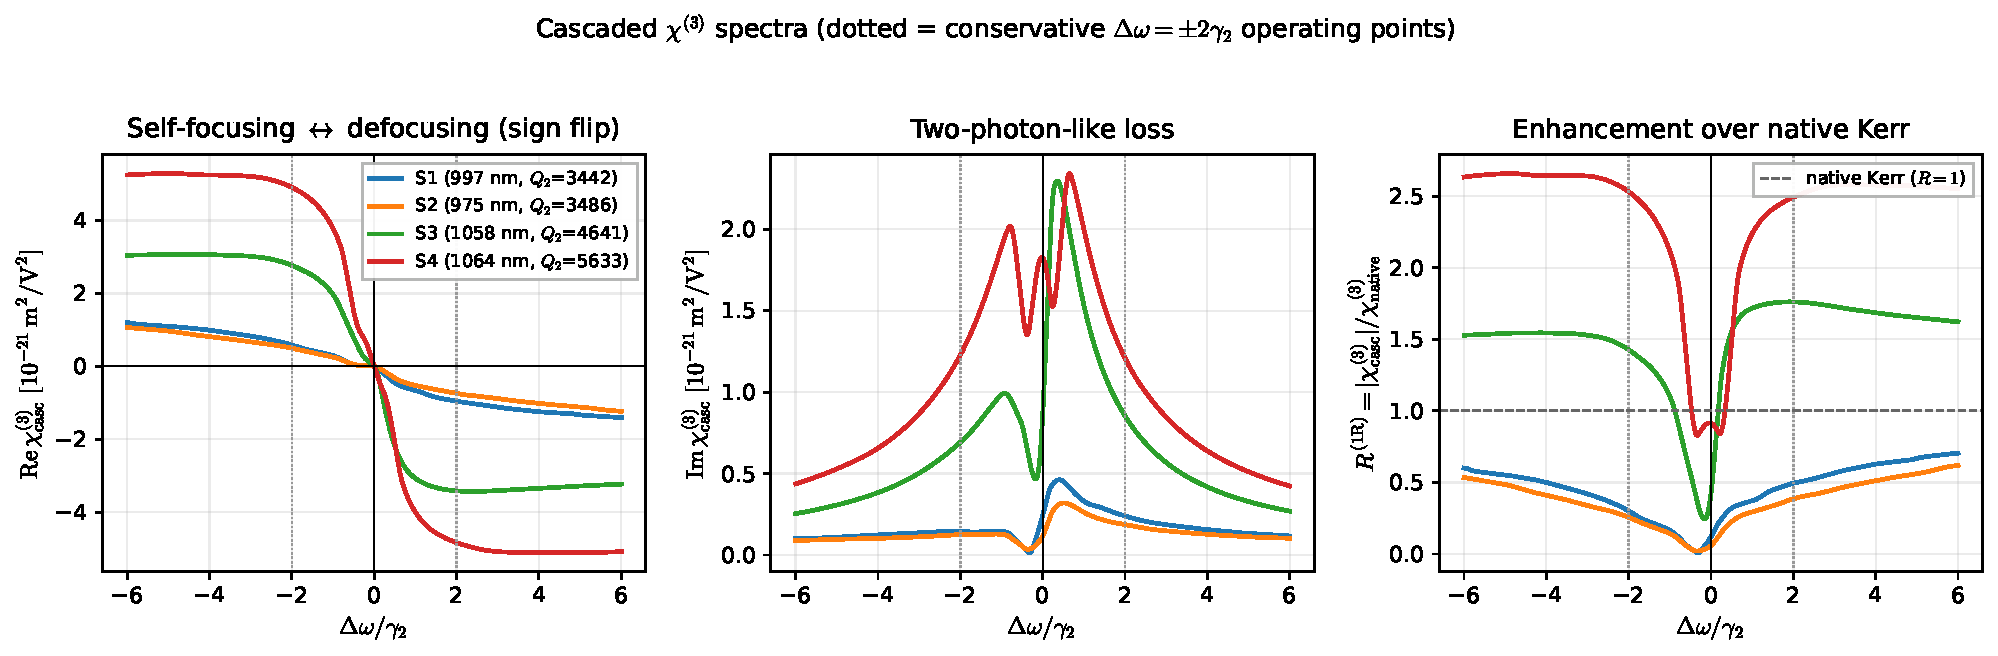
\includegraphics[width=\textwidth]{sample_chi3_spectra.pdf}
  \caption{Cascaded $\chithree$ versus SH detuning $\Dom/\gamma_2$ for all four
  samples. (a)~$\mathrm{Re}\,\chicasc$ flips sign at $\Dom=0$ (self-focusing for
  $\Dom<0$, defocusing for $\Dom>0$). (b)~$\mathrm{Im}\,\chicasc$ (two-photon-like
  loss). (c)~$R^{(1\mathrm R)}=|\chicasc|/\chithree_{\rm native}$; all four
  samples clear the native-Kerr line, S3 and S4 by $7$--$10\times$. Dotted:
  conservative $\Dom=\pm2\gamma_2$.}
  \label{fig:spectra}
\end{figure}

\paragraph{Sign flip.}
$\mathrm{Re}\,\chicasc\propto-\Dom$: a single metasurface delivers self-focusing,
self-defocusing, or exact cancellation of the native Kerr by choice of $\Dom$
(pump wavelength or post-fab SH trimming).

\paragraph{Loss peaks off resonance.}
Because the spatial overlap collapses at the exact SH resonance (a Fano feature in
the COMSOL data), $\mathrm{Im}\,\chicasc$ does \emph{not} peak at $\Dom=0$ as the
constant-$\eta$ model predicts, but at finite detuning --- a data-driven refinement
of the note. The same effect makes $R^{(1\mathrm R)}$ dip near $\Dom=0$ and rise
into the wings (Fig.~\ref{fig:spectra}c, \ref{fig:optimal}).

% =====================================================================
\section{Overlap-limited enhancement and bandwidth}
\label{sec:eta}

\begin{figure}[H]
  \centering
  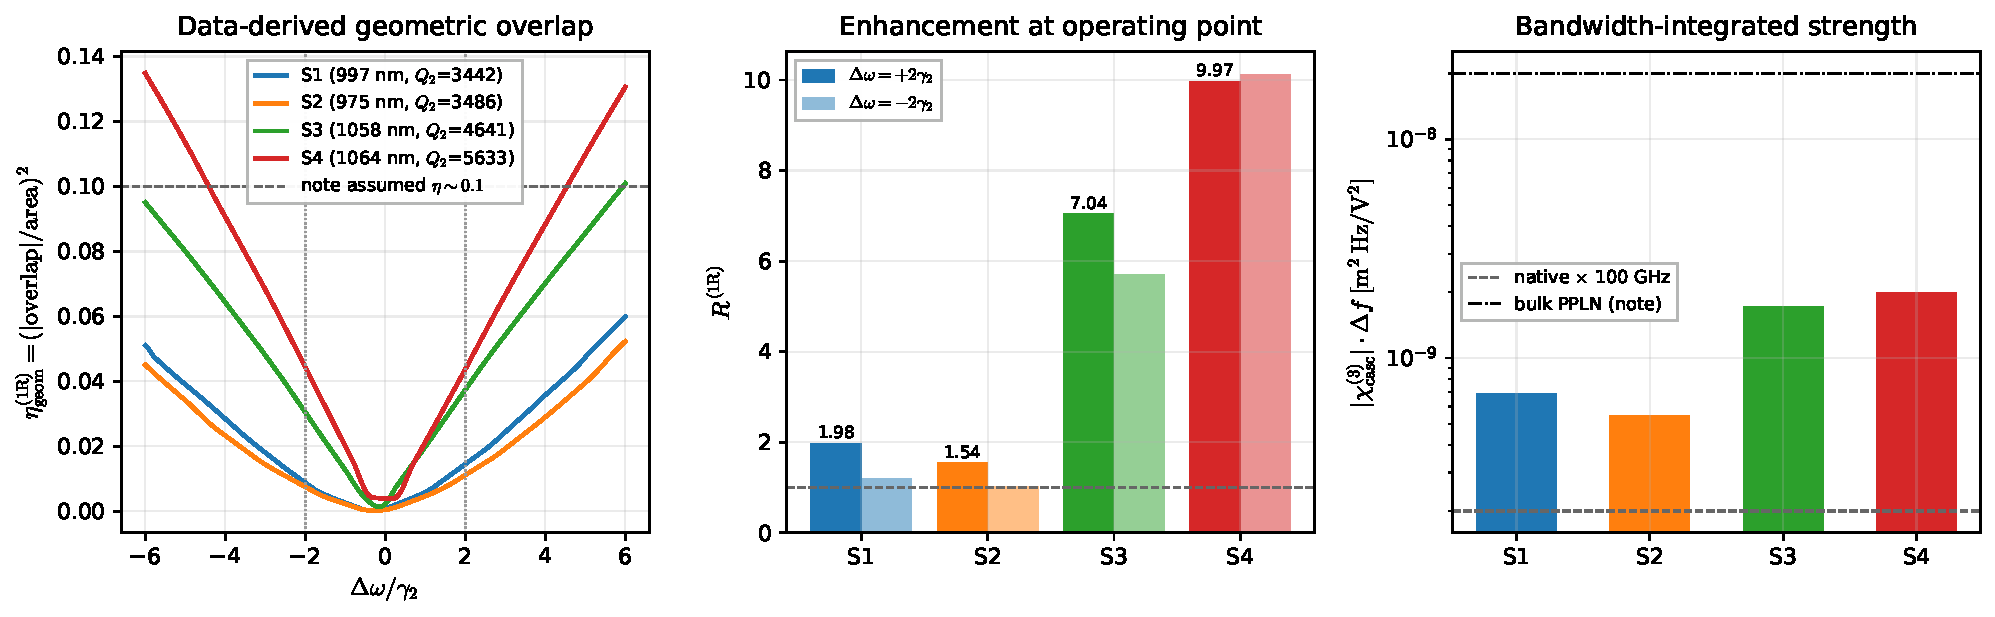
\includegraphics[width=\textwidth]{sample_eta_and_ranking.pdf}
  \caption{(a)~Data-derived $\etag(\Dom)=(|\text{overlap}|/A)^2$; all samples sit
  well below the note's assumed $0.1$ at $\pm2\gamma_2$ and collapse at $\Dom=0$.
  (b)~$R^{(1\mathrm R)}$ at $\Dom=\pm2\gamma_2$. (c)~Bandwidth-integrated strength
  $|\chicasc|\!\cdot\!\Delta f$, versus native$\times100\,$GHz and bulk PPLN.}
  \label{fig:eta}
\end{figure}

\paragraph{Ranking.}
$R^{(1\mathrm R)} =$ S4~$9.97 >$ S3~$7.04 >$ S1~$1.98 >$ S2~$1.54$. All four
exceed native LiNbO$_3$ Kerr; S3 and S4 by a wide margin. The binding constraint is the overlap:
$\etag=0.011$--$0.044$, a factor $2$--$10$ below the $\sim\!0.1$ assumed in the
note (\S\ref{sec:rules}, R1).

\paragraph{Bandwidth-integrated strength.}
Even the best sample sits $\sim\!10$--$50\times$ below bulk PPLN (depending on the
bulk bandwidth assumed, $2$--$10$\,THz) in
$|\chicasc|\!\cdot\!\Delta f$. The metasurface case is chip-scale form factor and
CW-threshold operation, not raw integrated nonlinear strength.

% =====================================================================
\section{Optimal detuning}
\label{sec:optimal}

\begin{figure}[H]
  \centering
  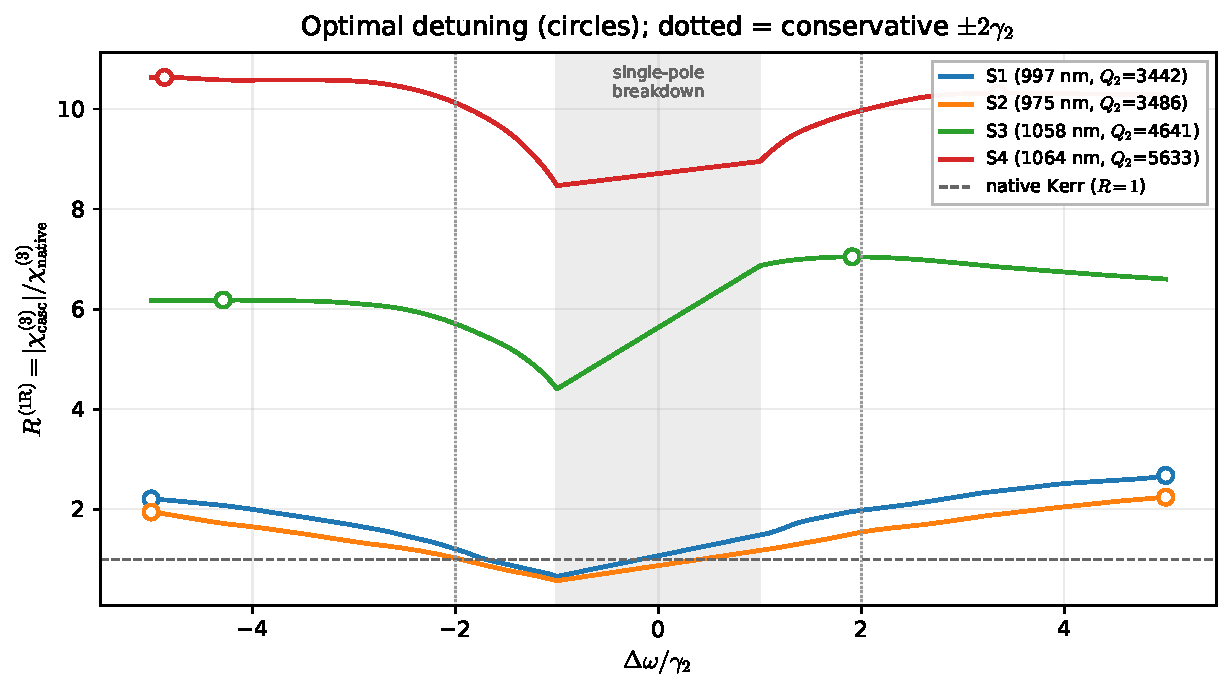
\includegraphics[width=0.85\textwidth]{sample_optimal_detuning.pdf}
  \caption{$R^{(1\mathrm R)}(\Dom)$ with the per-branch optima (circles) and the
  conservative $\pm2\gamma_2$ points (dotted). $R$ dips inside the
  $|\Dom|<\gamma_2$ single-pole breakdown band (shaded) and forms a broad plateau
  in the wings.}
  \label{fig:optimal}
\end{figure}

Scanning $\Dom$ over the validity window $|\Dom|\in[1,5]\gamma_2$ with the
data-derived $\etag(\Dom)$:

\begin{table}[H]
  \centering
  \caption{Optimal detuning per sample (best $|\chicasc|$ on each branch) versus
  the conservative $+2\gamma_2$ point.}
  \label{tab:optimal}
  \small
  \begin{tabular}{lccc}
    \toprule
    S & best defocus ($\Dom>0$) & best focus ($\Dom<0$) & gain over $+2\gamma_2$ \\
    \midrule
    1 & $+5\gamma_2$, $R\,2.67$   & $-5\gamma_2$, $R\,2.21$   & $\times1.35$ \\
    2 & $+5\gamma_2$, $R\,2.24$   & $-5\gamma_2$, $R\,1.94$   & $\times1.45$ \\
    3 & $+1.9\gamma_2$, $R\,7.05$ & $-4.3\gamma_2$, $R\,6.18$ & $\times1.00$ \\
    4 & $+3.3\gamma_2$, $R\,10.3$ & $-4.9\gamma_2$, $R\,10.6$ & $\times1.04$ \\
    \bottomrule
  \end{tabular}
\end{table}

\paragraph{Takeaway.}
Detuning is \emph{not} the lever. For the two useful samples the conservative
$\Dom=2\gamma_2$ is already within $\sim\!5\%$ of the achievable optimum; operating
closer ($|\Dom|<\gamma_2$) loses, because the overlap collapses there and the
single-pole/adiabatic model breaks. The weak samples cannot be detuned past native
Kerr at any point in the trusted window.

% =====================================================================
\section{Feasibility: single-pass phase and saturable absorption}
\label{sec:feasibility}

The single-pass per-photon Kerr phase and intensity-dependent loss are
(note Eqs.~\texttt{phi-1R}, \texttt{Im-chi3-1R})
\begin{equation}
  \varphi_{\rm NL}^{(1\mathrm R)} = \frac{3\omega_1}{2 c\,n_1}\,
        \mathrm{Re}\,\chicasc\,|\Eloc|^2 L_{\rm meta}\,,
  \qquad
  \left|\frac{\Delta T}{T}\right| = \frac{3\omega_1}{c\,n_1}\,
        \mathrm{Im}\,\chicasc\,|\Eloc|^2 L_{\rm meta}\,,
\end{equation}
with $|\Eloc|^2 = 2T_{\rm geom}^2 I_{\rm in}/(\eps_0 c\,n_1^2)$ and
$T_{\rm geom}=1$ (baseline).

\begin{figure}[H]
  \centering
  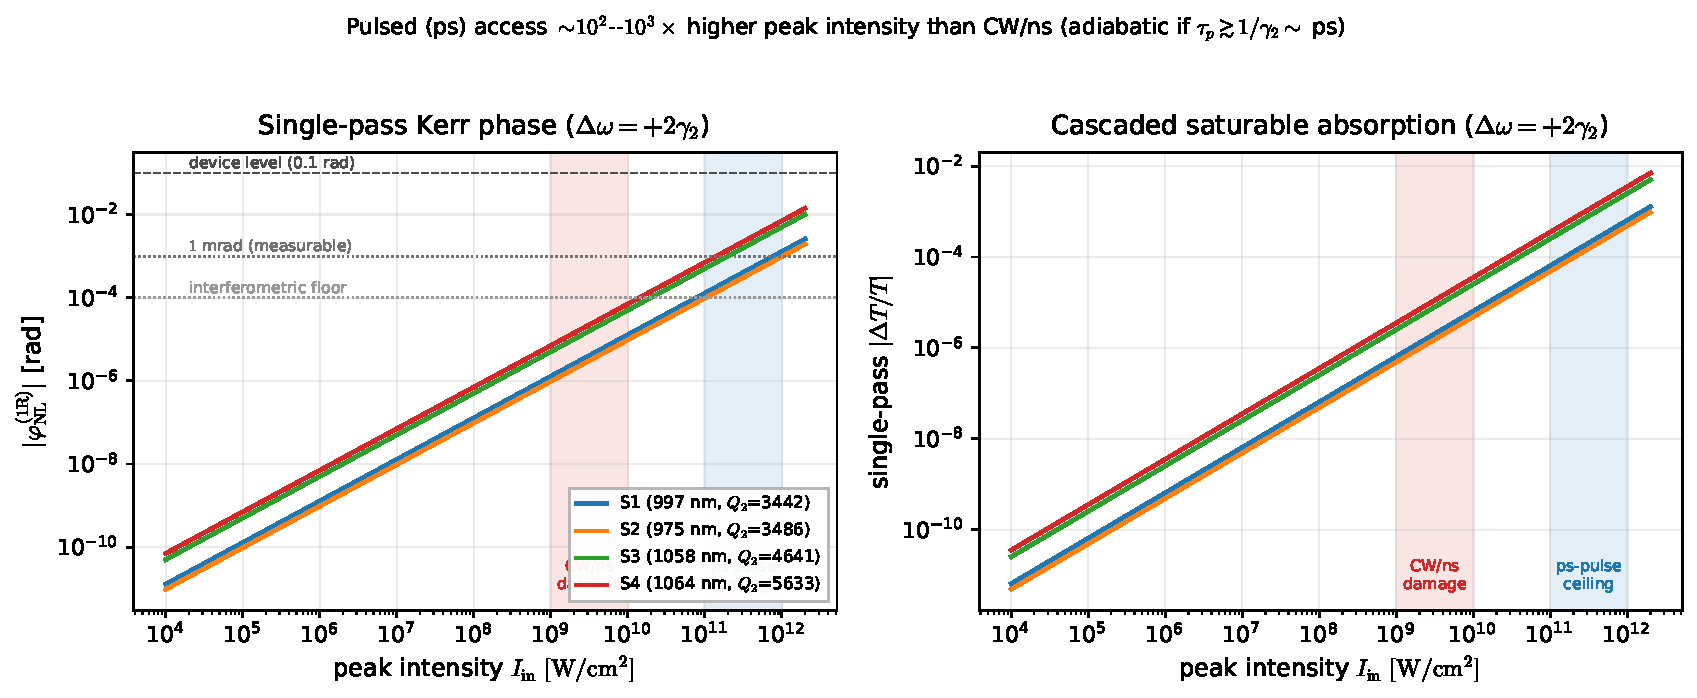
\includegraphics[width=\textwidth]{sample_feasibility.pdf}
  \caption{(a)~Single-pass Kerr phase $|\varphi_{\rm NL}|$ and (b)~saturable
  absorption $|\Delta T/T|$ vs.\ peak intensity at $\Dom=+2\gamma_2$. Shaded: the
  CW/ns damage band (1--10\,GW/cm$^2$, red) and the ps-pulse fluence ceiling
  ($\sim\!0.1$--$1$\,TW/cm$^2$, blue); the device level (0.1\,rad), 1\,mrad, and the
  interferometric floor are marked.}
  \label{fig:feasibility}
\end{figure}

\paragraph{CW: nothing observable.}
At the CW/ns damage threshold the best sample reaches only
$\varphi_{\rm NL}\!\sim\!10^{-4}$\,rad, and CW operation is anyway capped far lower by
green-SH photorefractive damage. No CW Kerr nonlinearity is observable; removing the
FM resonance removes the $Q_1^2$ build-up, as the note predicted.

\paragraph{Pulsed (ps): the $\chithree$ becomes measurable.}
Pulsed pumping helps substantially. It accesses $10^2$--$10^3\times$ higher peak
intensity \emph{and} sidesteps the CW photorefractive limit, lifting the phase to
$\sim$mrad and $\Delta T/T$ to $\sim\!10^{-3}$ --- enough to \emph{measure} the
$\chithree$, though still $\ll\!0.1$\,rad (no device). Power cannot recover the lost
$Q_1^2$. These estimates are quasi-static; since the experimental $\tau_p\!\sim\!1$--$3$\,ps
is comparable to the SH lifetime we test them with a time-domain pulse simulation
(\S\ref{sec:pulsed}).

% =====================================================================
\section{Time-domain pulse simulation}
\label{sec:pulsed}

Since $\tau_p\!\sim\!1$--$3$\,ps is comparable to the SH lifetime
$1/\gamma_2=0.9$--$1.6$\,ps, we integrate the actual SH-only TCMT (note Eq.~\texttt{a2-1R})
with the FM responding instantaneously, so the drive follows the pulse intensity envelope:
\begin{equation}
  \dot a_2 = (i\Dom - \tfrac{\gamma_2}{2})\,a_2 + i\,\beta(t),
  \qquad \beta(t)\propto |E_{\rm loc}(t)|^2 \propto I(t).
\end{equation}

\begin{figure}[H]
  \centering
  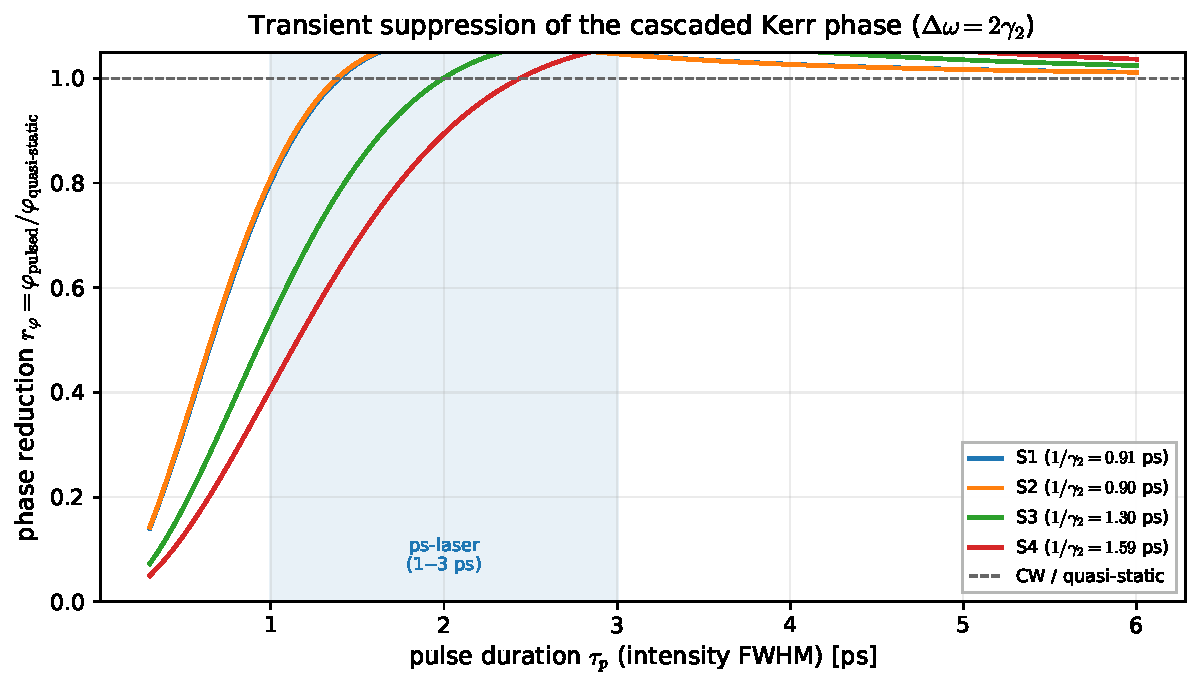
\includegraphics[width=0.5\textwidth]{sample_pulsed_reduction.pdf}\hfill
  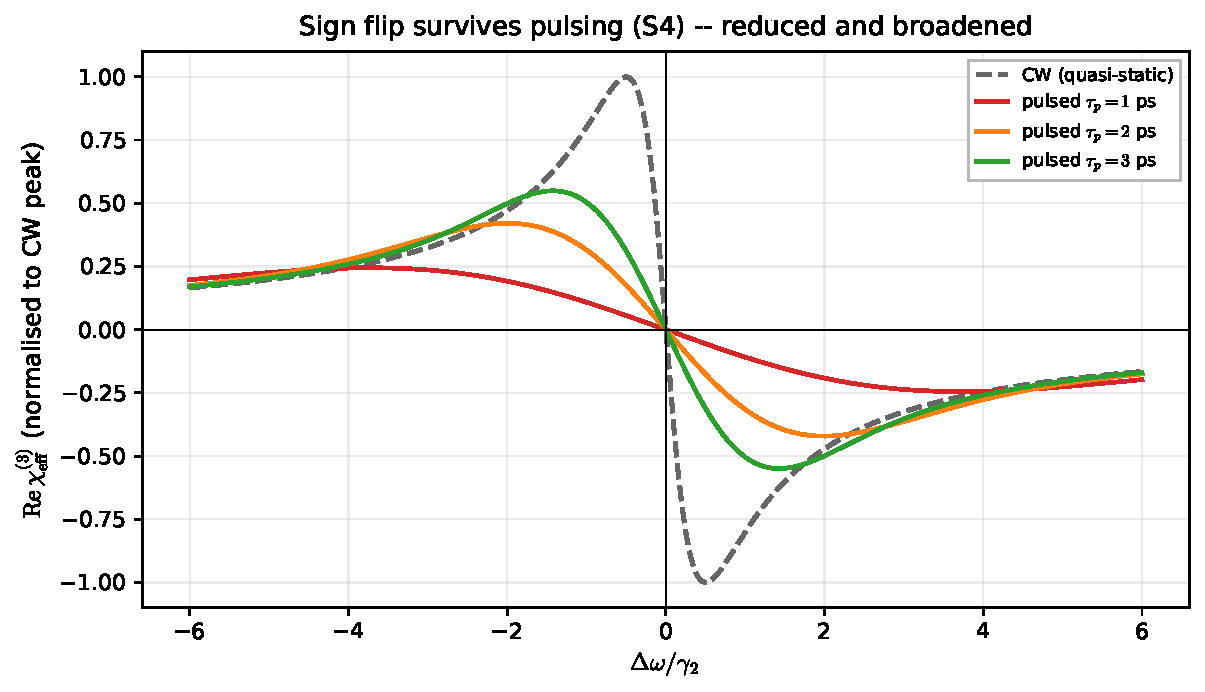
\includegraphics[width=0.49\textwidth]{sample_pulsed_signflip.pdf}
  \caption{Left: nonlinear-phase reduction
  $r_\varphi=\varphi_{\rm pulsed}/\varphi_{\rm quasi\text{-}static}$ vs pulse duration
  (1--3\,ps experimental band shaded). Right: the cascaded $\mathrm{Re}\,\chicasc$ sign
  flip survives pulsing (reduced and spectrally broadened, still flips at $\Dom=0$).}
  \label{fig:pulsed}
\end{figure}

\paragraph{The right observable.}
The \emph{energy}-integrated nonlinear phase is conserved for any pulse length (a sum
rule --- the SH delivers its full action, just spread over $\sim\!1/\gamma_2$). The
reduced, Z-scan-relevant quantity is the $I^2$-weighted / peak phase.

\paragraph{Result.}
At $\Dom=2\gamma_2$ the phase reduction is $r_\varphi(\tau_p\!=\!1\,{\rm ps})=0.80$
(S1/S2), $0.54$ (S3), $\mathbf{0.41}$ (S4), rising to $r_\varphi\!\approx\!0.9$--$1.07$ for
$\tau_p\!\geq\!2$\,ps (slight resonant overshoot). \textbf{The quasi-static estimate
holds for $\tau_p\!\gtrsim\!2$\,ps}; the penalty bites only at 1\,ps on the highest-$Q$
samples ($\sim\!2.5\times$ on S4). \textbf{Use $\tau_p\!\gtrsim\!2$\,ps.} The sign flip
survives, so the sign-flip experiment is robust at ps durations.

% =====================================================================
\section{FWM and SHG conversion}
\label{sec:fwmshg}

\begin{figure}[H]
  \centering
  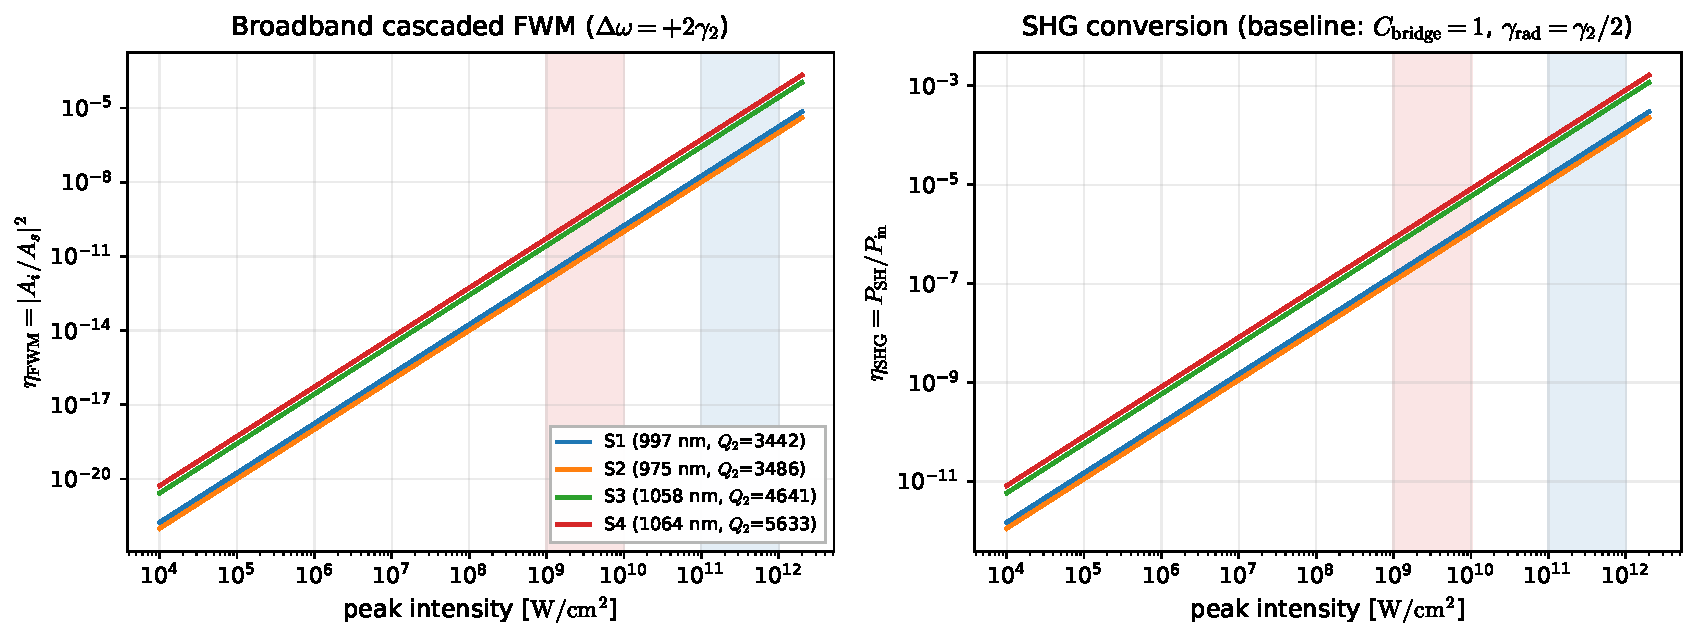
\includegraphics[width=\textwidth]{sample_fwm_shg.pdf}
  \caption{(a)~Broadband (phase-matching-free) cascaded FWM efficiency
  $\eta_{\rm FWM}=|A_i/A_s|^2$ and (b)~SHG conversion $\eta_{\rm SHG}=
  P_{\rm SH}/P_{\rm in}$ versus intensity at $\Dom=+2\gamma_2$. SHG is an
  order-of-magnitude baseline ($C_{\rm bridge}=1$, $\gamma_{\rm rad}=\gamma_2/2$).}
  \label{fig:fwmshg}
\end{figure}

\paragraph{FWM.}
Efficiency reaches $\sim\!10^{-4}$ only at the damage threshold; the sub-wavelength
thickness makes it phase-matching-free (full $\gamma_2$ bandwidth), useful as a
\emph{diagnostic} of $\chicasc$ rather than as a device.

\paragraph{SHG --- calibration only, not a target.}
SHG is a $\chitwo$ process and \emph{not} an objective of this $\chithree$ study. We
use it only because it shares the same overlap and SH resonance: measuring
$\eta_{\rm SHG}$ ($\sim\!10^{-7}$--$10^{-6}$ at 1\,GW/cm$^2$ baseline; $2\times$ the
pre-October-2026 values, after correcting the SH stored-energy bookkeeping) vs.\ detuning and power
\emph{pins the absolute $\chicasc$ scale} (the normalisation bridge, \S\ref{sec:open})
and validates the cascade's first ($\chitwo$) step.

\paragraph{Measuring the sign flip (the $\chithree$ observable).}
Pump at $\omega_1$ (always); scan the pump \emph{wavelength} so its \emph{generated}
harmonic $2\omega_1$ crosses the SH resonance $\omega_2$ ($\Dom=2\omega_1-\omega_2:-\!\to\!+$).
A closed-aperture Z-scan at each wavelength reads the sign of $n_2$ from the trace
ordering --- valley$\to$peak $=$ self-focusing ($n_2\!>\!0$), peak$\to$valley $=$
defocusing; the cascade is \textbf{odd in $\Dom$} and flips at $\Dom=0$ (Fig.~\ref{fig:spectra}a).
Native LiNbO$_3$ Kerr is a constant positive background, so a \emph{full} reversal of
the total $n_2$ needs $R>1$ (all four samples; S3/S4 with a wide margin); regardless, isolate the cascade as the
\textbf{antisymmetric-in-$\Dom$} component. Only $\sim\!1$\,nm of pump tuning spans
$\pm3\gamma_2$ at $Q_2\!\approx\!5000$. Equivalent probes: SPM/XPM spectral blue/red
asymmetry, or spectral interferometry for the signed phase.

% =====================================================================
\section{Observable verdict}
\label{sec:verdict}

\begin{table}[H]
  \centering
  \caption{Which effects are reasonable to observe with these samples.}
  \label{tab:verdict}
  \small
  \setlength{\tabcolsep}{5pt}
  \begin{tabular}{@{}p{4.5cm}p{3.6cm}p{4.7cm}@{}}
    \toprule
    Effect & Status in SH-only & Observable here? \\
    \midrule
    Sign flip (focus$\leftrightarrow$defocus) & $\chithree$, dispersive shape & \textbf{Yes, qualitatively} (scale-robust) \\
    $\chicasc$ / $R$ (material)      & material property       & Indirect; S3/S4 best ($R\,7$--$10$) \\
    Per-photon Kerr phase $\varphi_{\rm NL}$  & single-pass     & Only pulsed, $\sim$mrad; $\ll0.1$\,rad \\
    Saturable absorption $\Delta T/T$ & single-pass Im $\chithree$ & Only pulsed ($\sim\!10^{-3}$) \\
    Broadband FWM                    & single-pass             & Pulsed diagnostic \\
    SHG conversion efficiency       & $\chitwo$ (out of scope) & Calibration of $\chicasc$ scale only \\
    Bistability, switching, limiter, AM modulator & \emph{die} (no FM cavity) & No, at any power \\
    \bottomrule
  \end{tabular}
\end{table}

% =====================================================================
\section{Design rules for the optimal device}
\label{sec:rules}

\begin{enumerate}[label=\textbf{R\arabic*.},leftmargin=2.6em]
  \item \textbf{Maximise the nonlinear overlap (dominant, linear lever).}
        $\chicasc\propto\etag=|\text{overlap}|^2$. The samples sit at
        $|\text{overlap}|\!\approx\!0.10$--$0.21$; S4 already reaches $R\approx10$ at
        $|\text{overlap}|\!\approx\!0.21$; at S4's $Q$, $R=20$ needs $\approx\!0.30$ and
        $R=40$ needs $\approx\!0.42$. Target
        $|\text{overlap}|\!\gtrsim\!0.3$ at the operating detuning via stronger
        qBIC asymmetry (staying absorption-limited, where $|\text{overlap}|^2Q$
        grows with asymmetry), sub-domain (unit-cell) poling of $\chitwo$, or
        pump-near-field shaping.
  \item \textbf{Fix the detuning at $\Dom\approx2\gamma_2$; don't chase it}
        (\S\ref{sec:optimal}): within $\sim\!5\%$ of optimal, TPA penalty
        $(\gamma_2/2\Dom)^2=1/16$, adiabatic approximation clean.
  \item \textbf{Push $Q_2$ with diminishing returns and a disorder floor.}
        $\chicasc\propto Q_2$, but only one power of $Q$ helps in 1R, bandwidth
        $\propto1/Q_2$, and the array linewidth must beat disorder
        ($\sigma_\omega/\omega\lesssim1/Q_2\!\approx\!2\times10^{-4}$ at
        $Q_2=5000$). Verify the \emph{array} (not single-element) $Q$.
  \item \textbf{Thicker LiNbO$_3$.} Single-pass $\varphi_{\rm NL}$, $\Delta T/T$,
        FWM all $\propto L_{\rm meta}$ (not $\chicasc$ itself).
  \item \textbf{Pump with ps pulses; use MgO-doped LiNbO$_3$.} The SH is green
        (488--532\,nm), where CW is photorefractively limited; ps pulses
        ($\tau_p\!\gtrsim\!1/\gamma_2\!\sim\!$ps) give $10^2$--$10^3\times$ more peak
        intensity and escape that limit, lifting the $\chithree$ signals into the
        measurable range ($\sim$mrad).
  \item \textbf{Confirm $Q$ is the loaded value.} An FWHM read of the SH dip gives
        $\approx\!0.6\times$ the quoted $Q$; the model needs the total $\gamma_2$
        and $\chicasc\propto Q_2$.
  \item \textbf{For a CW Kerr \emph{device}, go doubly-resonant.} Even fully
        overlap-optimised, the SH-only per-photon phase lacks the $Q_1^2$ FM-cavity
        build-up and stays $\mu$rad-class. SH-only's best roles are a $\chithree$
        \emph{diagnostic} (sign flip + FWM; SHG only to calibrate the scale) and
        \emph{materials-level} $\chithree$; a bistability/switching device needs the
        FM qBIC added back.
  \item \textbf{Match sample to pump} ($\lambda_1=975$--$1064\,$nm; S4 $=$ Nd:YAG)
        and trim the SH resonance post-fabrication to set $\Dom$.
\end{enumerate}

% =====================================================================
\section{Verification}
\label{sec:verify}

All formulae were re-derived from the note and cross-checked two independent ways
(\texttt{cascaded\_chi3/sample\_optimal.py} and an independent reviewer): the
prefactor-free identity $\mathrm{Re}/\mathrm{Im}\,\chicasc=-2(\Dom/\gamma_2)$ holds
exactly; the lineshape matches the dimensionless adiabatic forms of
\texttt{analytic.py} to $2.5\times10^{-16}$; units reduce to m$^2$/V$^2$
($\chicasc$) and rad ($\varphi_{\rm NL}$); and the sample-4 spot value
$|\chicasc|=1.99\times10^{-20}$, $R=9.97$ was reproduced by hand. The Boyd
degeneracy factors (3 for SPM/phase, $2\times$ for loss-vs-phase, cubic pump in
FWM), the $\eps_0$ cancellation, and the squared overlap in $\etag$ are all
correct. \textbf{No discrepancies.}

% =====================================================================
\section{Open items and the absolute scale}
\label{sec:open}

Rankings, lineshapes, sign-flip, and $Q/\eta$ scalings are robust. Absolute
magnitudes ($\chicasc$, $\varphi_{\rm NL}$, $\Delta T/T$, $\eta_{\rm FWM}$,
$\eta_{\rm SHG}$) scale with the normalisation bridge $C_{\rm bridge}$ (the
2-D-overlap $\to$ 3-D-Brillouin mapping, baseline 1), with $|\chitwo|^2$, and with
$1/\chithree_{\rm native}$ --- all $\mathcal{O}(1)$ at present. A single absolute
SHG-efficiency datum (one full nonlinear simulation) pins the bridge; the full
open-question list is in \texttt{SH\_only\_designer\_questions.md}. Other open items: the undocumented
\texttt{symmetry} field, the loaded-vs-intrinsic $Q$, the radiative/absorptive
split, and refined $d_{33}/\chithree_{\rm native}$ at $\sim\!1\,\mu$m.

% =====================================================================
\section{Reproduce}
\label{sec:code}

Run \texttt{conda run -n ml\_base python cascaded\_chi3/<script>.py} with
\texttt{<script>} one of:
\begin{itemize}[nosep]
  \item \texttt{sample\_params} --- parameters + consistency checks;
  \item \texttt{sample\_effects} --- effects + figures;
  \item \texttt{sample\_optimal} --- cross-checks + optimal detuning;
  \item \texttt{sample\_pulsed} --- time-domain pulsed TCMT.
\end{itemize}
Figures are written to \texttt{cascaded\_chi3/figures/samples/}. Companion
markdown: \texttt{SH\_only\_sample\_parameters.md} (extraction),
\texttt{SH\_only\_sample\_analysis.md} (analysis),
\texttt{SH\_only\_designer\_questions.md} (designer queries).

\end{document}
